% Created by tikzDevice version 0.12.6 on 2025-04-07 03:04:37
% !TEX encoding = UTF-8 Unicode
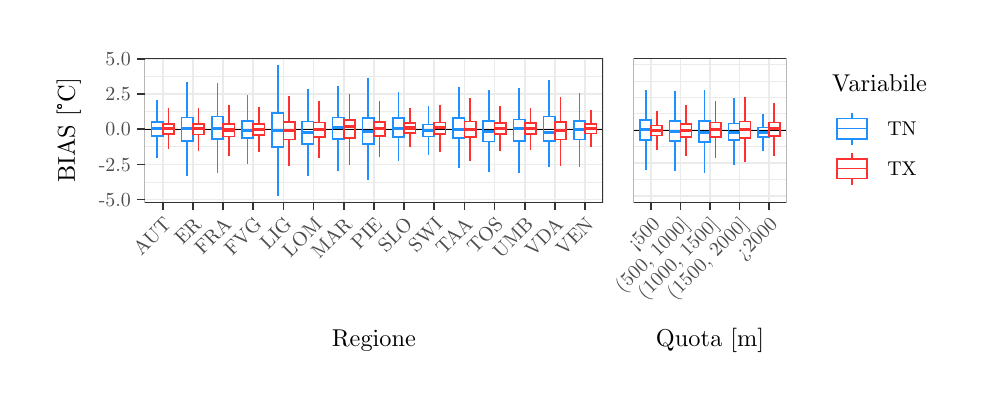
\begin{tikzpicture}[x=1pt,y=1pt]
\definecolor{fillColor}{RGB}{255,255,255}
\path[use as bounding box,fill=fillColor] (0,0) rectangle (341.43,128.04);
\begin{scope}
\path[clip] (  0.00,  0.00) rectangle (341.43,128.04);
\definecolor{drawColor}{RGB}{255,255,255}

\path[draw=drawColor,line width= 0.6pt,line join=round,line cap=round,fill=fillColor] (  0.00,  0.00) rectangle (341.43,128.04);
\end{scope}
\begin{scope}
\path[clip] (  5.50,  5.50) rectangle (213.45,122.54);
\definecolor{drawColor}{RGB}{255,255,255}
\definecolor{fillColor}{RGB}{255,255,255}

\path[draw=drawColor,line width= 0.6pt,line join=round,line cap=round,fill=fillColor] (  5.50,  5.50) rectangle (213.45,122.54);
\end{scope}
\begin{scope}
\path[clip] (213.45,  5.50) rectangle (335.93,122.54);
\definecolor{drawColor}{RGB}{255,255,255}
\definecolor{fillColor}{RGB}{255,255,255}

\path[draw=drawColor,line width= 0.6pt,line join=round,line cap=round,fill=fillColor] (213.45,  5.50) rectangle (335.93,122.54);
\end{scope}
\begin{scope}
\path[clip] ( 42.24, 64.87) rectangle (207.95,117.04);
\definecolor{fillColor}{RGB}{255,255,255}

\path[fill=fillColor] ( 42.24, 64.87) rectangle (207.95,117.04);
\definecolor{drawColor}{gray}{0.92}

\path[draw=drawColor,line width= 0.3pt,line join=round] ( 42.24, 72.27) --
	(207.95, 72.27);

\path[draw=drawColor,line width= 0.3pt,line join=round] ( 42.24, 85.00) --
	(207.95, 85.00);

\path[draw=drawColor,line width= 0.3pt,line join=round] ( 42.24, 97.73) --
	(207.95, 97.73);

\path[draw=drawColor,line width= 0.3pt,line join=round] ( 42.24,110.46) --
	(207.95,110.46);

\path[draw=drawColor,line width= 0.6pt,line join=round] ( 42.24, 65.90) --
	(207.95, 65.90);

\path[draw=drawColor,line width= 0.6pt,line join=round] ( 42.24, 78.64) --
	(207.95, 78.64);

\path[draw=drawColor,line width= 0.6pt,line join=round] ( 42.24, 91.37) --
	(207.95, 91.37);

\path[draw=drawColor,line width= 0.6pt,line join=round] ( 42.24,104.10) --
	(207.95,104.10);

\path[draw=drawColor,line width= 0.6pt,line join=round] ( 42.24,116.83) --
	(207.95,116.83);

\path[draw=drawColor,line width= 0.6pt,line join=round] ( 48.78, 64.87) --
	( 48.78,117.04);

\path[draw=drawColor,line width= 0.6pt,line join=round] ( 59.69, 64.87) --
	( 59.69,117.04);

\path[draw=drawColor,line width= 0.6pt,line join=round] ( 70.59, 64.87) --
	( 70.59,117.04);

\path[draw=drawColor,line width= 0.6pt,line join=round] ( 81.49, 64.87) --
	( 81.49,117.04);

\path[draw=drawColor,line width= 0.6pt,line join=round] ( 92.39, 64.87) --
	( 92.39,117.04);

\path[draw=drawColor,line width= 0.6pt,line join=round] (103.29, 64.87) --
	(103.29,117.04);

\path[draw=drawColor,line width= 0.6pt,line join=round] (114.19, 64.87) --
	(114.19,117.04);

\path[draw=drawColor,line width= 0.6pt,line join=round] (125.10, 64.87) --
	(125.10,117.04);

\path[draw=drawColor,line width= 0.6pt,line join=round] (136.00, 64.87) --
	(136.00,117.04);

\path[draw=drawColor,line width= 0.6pt,line join=round] (146.90, 64.87) --
	(146.90,117.04);

\path[draw=drawColor,line width= 0.6pt,line join=round] (157.80, 64.87) --
	(157.80,117.04);

\path[draw=drawColor,line width= 0.6pt,line join=round] (168.70, 64.87) --
	(168.70,117.04);

\path[draw=drawColor,line width= 0.6pt,line join=round] (179.61, 64.87) --
	(179.61,117.04);

\path[draw=drawColor,line width= 0.6pt,line join=round] (190.51, 64.87) --
	(190.51,117.04);

\path[draw=drawColor,line width= 0.6pt,line join=round] (201.41, 64.87) --
	(201.41,117.04);
\definecolor{drawColor}{RGB}{0,0,0}

\path[draw=drawColor,line width= 0.1pt,line join=round] ( 42.24, 91.37) -- (207.95, 91.37);
\definecolor{drawColor}{RGB}{30,144,255}

\path[draw=drawColor,line width= 0.6pt,line join=round] ( 46.74, 94.07) -- ( 46.74,101.75);

\path[draw=drawColor,line width= 0.6pt,line join=round] ( 46.74, 88.82) -- ( 46.74, 80.95);

\path[draw=drawColor,line width= 0.6pt] ( 44.70, 94.07) --
	( 44.70, 88.82) --
	( 48.78, 88.82) --
	( 48.78, 94.07) --
	( 44.70, 94.07) --
	cycle;

\path[draw=drawColor,line width= 1.1pt] ( 44.70, 91.72) -- ( 48.78, 91.72);
\definecolor{drawColor}{RGB}{255,48,48}

\path[draw=drawColor,line width= 0.6pt,line join=round] ( 50.83, 93.32) -- ( 50.83, 98.94);

\path[draw=drawColor,line width= 0.6pt,line join=round] ( 50.83, 89.58) -- ( 50.83, 84.06);

\path[draw=drawColor,line width= 0.6pt] ( 48.78, 93.32) --
	( 48.78, 89.58) --
	( 52.87, 89.58) --
	( 52.87, 93.32) --
	( 48.78, 93.32) --
	cycle;

\path[draw=drawColor,line width= 1.1pt] ( 48.78, 91.45) -- ( 52.87, 91.45);
\definecolor{drawColor}{RGB}{30,144,255}

\path[draw=drawColor,line width= 0.6pt,line join=round] ( 57.64, 95.62) -- ( 57.64,108.34);

\path[draw=drawColor,line width= 0.6pt,line join=round] ( 57.64, 87.09) -- ( 57.64, 74.54);

\path[draw=drawColor,line width= 0.6pt] ( 55.60, 95.62) --
	( 55.60, 87.09) --
	( 59.69, 87.09) --
	( 59.69, 95.62) --
	( 55.60, 95.62) --
	cycle;

\path[draw=drawColor,line width= 1.1pt] ( 55.60, 91.62) -- ( 59.69, 91.62);
\definecolor{drawColor}{RGB}{255,48,48}

\path[draw=drawColor,line width= 0.6pt,line join=round] ( 61.73, 93.30) -- ( 61.73, 99.14);

\path[draw=drawColor,line width= 0.6pt,line join=round] ( 61.73, 89.39) -- ( 61.73, 83.61);

\path[draw=drawColor,line width= 0.6pt] ( 59.69, 93.30) --
	( 59.69, 89.39) --
	( 63.77, 89.39) --
	( 63.77, 93.30) --
	( 59.69, 93.30) --
	cycle;

\path[draw=drawColor,line width= 1.1pt] ( 59.69, 91.46) -- ( 63.77, 91.46);
\definecolor{drawColor}{RGB}{30,144,255}

\path[draw=drawColor,line width= 0.6pt,line join=round] ( 68.54, 95.93) -- ( 68.54,108.05);

\path[draw=drawColor,line width= 0.6pt,line join=round] ( 68.54, 87.81) -- ( 68.54, 75.64);

\path[draw=drawColor,line width= 0.6pt] ( 66.50, 95.93) --
	( 66.50, 87.81) --
	( 70.59, 87.81) --
	( 70.59, 95.93) --
	( 66.50, 95.93) --
	cycle;

\path[draw=drawColor,line width= 1.1pt] ( 66.50, 91.47) -- ( 70.59, 91.47);
\definecolor{drawColor}{RGB}{255,48,48}

\path[draw=drawColor,line width= 0.6pt,line join=round] ( 72.63, 93.27) -- ( 72.63,100.13);

\path[draw=drawColor,line width= 0.6pt,line join=round] ( 72.63, 88.66) -- ( 72.63, 81.75);

\path[draw=drawColor,line width= 0.6pt] ( 70.59, 93.27) --
	( 70.59, 88.66) --
	( 74.68, 88.66) --
	( 74.68, 93.27) --
	( 70.59, 93.27) --
	cycle;

\path[draw=drawColor,line width= 1.1pt] ( 70.59, 91.07) -- ( 74.68, 91.07);
\definecolor{drawColor}{RGB}{30,144,255}

\path[draw=drawColor,line width= 0.6pt,line join=round] ( 79.45, 94.29) -- ( 79.45,103.59);

\path[draw=drawColor,line width= 0.6pt,line join=round] ( 79.45, 88.09) -- ( 79.45, 78.83);

\path[draw=drawColor,line width= 0.6pt] ( 77.40, 94.29) --
	( 77.40, 88.09) --
	( 81.49, 88.09) --
	( 81.49, 94.29) --
	( 77.40, 94.29) --
	cycle;

\path[draw=drawColor,line width= 1.1pt] ( 77.40, 90.97) -- ( 81.49, 90.97);
\definecolor{drawColor}{RGB}{255,48,48}

\path[draw=drawColor,line width= 0.6pt,line join=round] ( 83.53, 93.28) -- ( 83.53, 99.33);

\path[draw=drawColor,line width= 0.6pt,line join=round] ( 83.53, 89.24) -- ( 83.53, 83.19);

\path[draw=drawColor,line width= 0.6pt] ( 81.49, 93.28) --
	( 81.49, 89.24) --
	( 85.58, 89.24) --
	( 85.58, 93.28) --
	( 81.49, 93.28) --
	cycle;

\path[draw=drawColor,line width= 1.1pt] ( 81.49, 91.26) -- ( 85.58, 91.26);
\definecolor{drawColor}{RGB}{30,144,255}

\path[draw=drawColor,line width= 0.6pt,line join=round] ( 90.35, 97.11) -- ( 90.35,114.67);

\path[draw=drawColor,line width= 0.6pt,line join=round] ( 90.35, 85.00) -- ( 90.35, 67.24);

\path[draw=drawColor,line width= 0.6pt] ( 88.30, 97.11) --
	( 88.30, 85.00) --
	( 92.39, 85.00) --
	( 92.39, 97.11) --
	( 88.30, 97.11) --
	cycle;

\path[draw=drawColor,line width= 1.1pt] ( 88.30, 90.79) -- ( 92.39, 90.79);
\definecolor{drawColor}{RGB}{255,48,48}

\path[draw=drawColor,line width= 0.6pt,line join=round] ( 94.44, 93.92) -- ( 94.44,103.38);

\path[draw=drawColor,line width= 0.6pt,line join=round] ( 94.44, 87.59) -- ( 94.44, 78.21);

\path[draw=drawColor,line width= 0.6pt] ( 92.39, 93.92) --
	( 92.39, 87.59) --
	( 96.48, 87.59) --
	( 96.48, 93.92) --
	( 92.39, 93.92) --
	cycle;

\path[draw=drawColor,line width= 1.1pt] ( 92.39, 90.82) -- ( 96.48, 90.82);
\definecolor{drawColor}{RGB}{30,144,255}

\path[draw=drawColor,line width= 0.6pt,line join=round] (101.25, 94.11) -- (101.25,105.85);

\path[draw=drawColor,line width= 0.6pt,line join=round] (101.25, 86.08) -- (101.25, 74.41);

\path[draw=drawColor,line width= 0.6pt] ( 99.20, 94.11) --
	( 99.20, 86.08) --
	(103.29, 86.08) --
	(103.29, 94.11) --
	( 99.20, 94.11) --
	cycle;

\path[draw=drawColor,line width= 1.1pt] ( 99.20, 90.00) -- (103.29, 90.00);
\definecolor{drawColor}{RGB}{255,48,48}

\path[draw=drawColor,line width= 0.6pt,line join=round] (105.34, 93.75) -- (105.34,101.44);

\path[draw=drawColor,line width= 0.6pt,line join=round] (105.34, 88.57) -- (105.34, 80.83);

\path[draw=drawColor,line width= 0.6pt] (103.29, 93.75) --
	(103.29, 88.57) --
	(107.38, 88.57) --
	(107.38, 93.75) --
	(103.29, 93.75) --
	cycle;

\path[draw=drawColor,line width= 1.1pt] (103.29, 91.14) -- (107.38, 91.14);
\definecolor{drawColor}{RGB}{30,144,255}

\path[draw=drawColor,line width= 0.6pt,line join=round] (112.15, 95.56) -- (112.15,107.02);

\path[draw=drawColor,line width= 0.6pt,line join=round] (112.15, 87.84) -- (112.15, 76.30);

\path[draw=drawColor,line width= 0.6pt] (110.11, 95.56) --
	(110.11, 87.84) --
	(114.19, 87.84) --
	(114.19, 95.56) --
	(110.11, 95.56) --
	cycle;

\path[draw=drawColor,line width= 1.1pt] (110.11, 91.88) -- (114.19, 91.88);
\definecolor{drawColor}{RGB}{255,48,48}

\path[draw=drawColor,line width= 0.6pt,line join=round] (116.24, 94.56) -- (116.24,103.92);

\path[draw=drawColor,line width= 0.6pt,line join=round] (116.24, 88.12) -- (116.24, 78.52);

\path[draw=drawColor,line width= 0.6pt] (114.19, 94.56) --
	(114.19, 88.12) --
	(118.28, 88.12) --
	(118.28, 94.56) --
	(114.19, 94.56) --
	cycle;

\path[draw=drawColor,line width= 1.1pt] (114.19, 92.20) -- (118.28, 92.20);
\definecolor{drawColor}{RGB}{30,144,255}

\path[draw=drawColor,line width= 0.6pt,line join=round] (123.05, 95.51) -- (123.05,109.74);

\path[draw=drawColor,line width= 0.6pt,line join=round] (123.05, 86.03) -- (123.05, 72.94);

\path[draw=drawColor,line width= 0.6pt] (121.01, 95.51) --
	(121.01, 86.03) --
	(125.10, 86.03) --
	(125.10, 95.51) --
	(121.01, 95.51) --
	cycle;

\path[draw=drawColor,line width= 1.1pt] (121.01, 90.52) -- (125.10, 90.52);
\definecolor{drawColor}{RGB}{255,48,48}

\path[draw=drawColor,line width= 0.6pt,line join=round] (127.14, 94.06) -- (127.14,101.59);

\path[draw=drawColor,line width= 0.6pt,line join=round] (127.14, 88.99) -- (127.14, 81.44);

\path[draw=drawColor,line width= 0.6pt] (125.10, 94.06) --
	(125.10, 88.99) --
	(129.18, 88.99) --
	(129.18, 94.06) --
	(125.10, 94.06) --
	cycle;

\path[draw=drawColor,line width= 1.1pt] (125.10, 91.44) -- (129.18, 91.44);
\definecolor{drawColor}{RGB}{30,144,255}

\path[draw=drawColor,line width= 0.6pt,line join=round] (133.95, 95.35) -- (133.95,104.90);

\path[draw=drawColor,line width= 0.6pt,line join=round] (133.95, 88.64) -- (133.95, 79.72);

\path[draw=drawColor,line width= 0.6pt] (131.91, 95.35) --
	(131.91, 88.64) --
	(136.00, 88.64) --
	(136.00, 95.35) --
	(131.91, 95.35) --
	cycle;

\path[draw=drawColor,line width= 1.1pt] (131.91, 91.76) -- (136.00, 91.76);
\definecolor{drawColor}{RGB}{255,48,48}

\path[draw=drawColor,line width= 0.6pt,line join=round] (138.04, 93.66) -- (138.04, 98.98);

\path[draw=drawColor,line width= 0.6pt,line join=round] (138.04, 90.08) -- (138.04, 84.75);

\path[draw=drawColor,line width= 0.6pt] (136.00, 93.66) --
	(136.00, 90.08) --
	(140.09, 90.08) --
	(140.09, 93.66) --
	(136.00, 93.66) --
	cycle;

\path[draw=drawColor,line width= 1.1pt] (136.00, 91.78) -- (140.09, 91.78);
\definecolor{drawColor}{RGB}{30,144,255}

\path[draw=drawColor,line width= 0.6pt,line join=round] (144.86, 93.10) -- (144.86, 99.69);

\path[draw=drawColor,line width= 0.6pt,line join=round] (144.86, 88.69) -- (144.86, 82.17);

\path[draw=drawColor,line width= 0.6pt] (142.81, 93.10) --
	(142.81, 88.69) --
	(146.90, 88.69) --
	(146.90, 93.10) --
	(142.81, 93.10) --
	cycle;

\path[draw=drawColor,line width= 1.1pt] (142.81, 90.87) -- (146.90, 90.87);
\definecolor{drawColor}{RGB}{255,48,48}

\path[draw=drawColor,line width= 0.6pt,line join=round] (148.94, 93.81) -- (148.94,100.11);

\path[draw=drawColor,line width= 0.6pt,line join=round] (148.94, 89.59) -- (148.94, 83.26);

\path[draw=drawColor,line width= 0.6pt] (146.90, 93.81) --
	(146.90, 89.59) --
	(150.99, 89.59) --
	(150.99, 93.81) --
	(146.90, 93.81) --
	cycle;

\path[draw=drawColor,line width= 1.1pt] (146.90, 91.82) -- (150.99, 91.82);
\definecolor{drawColor}{RGB}{30,144,255}

\path[draw=drawColor,line width= 0.6pt,line join=round] (155.76, 95.51) -- (155.76,106.53);

\path[draw=drawColor,line width= 0.6pt,line join=round] (155.76, 88.15) -- (155.76, 77.26);

\path[draw=drawColor,line width= 0.6pt] (153.71, 95.51) --
	(153.71, 88.15) --
	(157.80, 88.15) --
	(157.80, 95.51) --
	(153.71, 95.51) --
	cycle;

\path[draw=drawColor,line width= 1.1pt] (153.71, 91.36) -- (157.80, 91.36);
\definecolor{drawColor}{RGB}{255,48,48}

\path[draw=drawColor,line width= 0.6pt,line join=round] (159.85, 94.10) -- (159.85,102.54);

\path[draw=drawColor,line width= 0.6pt,line join=round] (159.85, 88.46) -- (159.85, 80.00);

\path[draw=drawColor,line width= 0.6pt] (157.80, 94.10) --
	(157.80, 88.46) --
	(161.89, 88.46) --
	(161.89, 94.10) --
	(157.80, 94.10) --
	cycle;

\path[draw=drawColor,line width= 1.1pt] (157.80, 91.27) -- (161.89, 91.27);
\definecolor{drawColor}{RGB}{30,144,255}

\path[draw=drawColor,line width= 0.6pt,line join=round] (166.66, 94.41) -- (166.66,105.61);

\path[draw=drawColor,line width= 0.6pt,line join=round] (166.66, 86.93) -- (166.66, 75.81);

\path[draw=drawColor,line width= 0.6pt] (164.62, 94.41) --
	(164.62, 86.93) --
	(168.70, 86.93) --
	(168.70, 94.41) --
	(164.62, 94.41) --
	cycle;

\path[draw=drawColor,line width= 1.1pt] (164.62, 90.50) -- (168.70, 90.50);
\definecolor{drawColor}{RGB}{255,48,48}

\path[draw=drawColor,line width= 0.6pt,line join=round] (170.75, 93.66) -- (170.75, 99.86);

\path[draw=drawColor,line width= 0.6pt,line join=round] (170.75, 89.52) -- (170.75, 83.34);

\path[draw=drawColor,line width= 0.6pt] (168.70, 93.66) --
	(168.70, 89.52) --
	(172.79, 89.52) --
	(172.79, 93.66) --
	(168.70, 93.66) --
	cycle;

\path[draw=drawColor,line width= 1.1pt] (168.70, 91.61) -- (172.79, 91.61);
\definecolor{drawColor}{RGB}{30,144,255}

\path[draw=drawColor,line width= 0.6pt,line join=round] (177.56, 94.88) -- (177.56,106.18);

\path[draw=drawColor,line width= 0.6pt,line join=round] (177.56, 87.08) -- (177.56, 75.61);

\path[draw=drawColor,line width= 0.6pt] (175.52, 94.88) --
	(175.52, 87.08) --
	(179.61, 87.08) --
	(179.61, 94.88) --
	(175.52, 94.88) --
	cycle;

\path[draw=drawColor,line width= 1.1pt] (175.52, 91.70) -- (179.61, 91.70);
\definecolor{drawColor}{RGB}{255,48,48}

\path[draw=drawColor,line width= 0.6pt,line join=round] (181.65, 93.55) -- (181.65, 99.17);

\path[draw=drawColor,line width= 0.6pt,line join=round] (181.65, 89.62) -- (181.65, 83.75);

\path[draw=drawColor,line width= 0.6pt] (179.61, 93.55) --
	(179.61, 89.62) --
	(183.69, 89.62) --
	(183.69, 93.55) --
	(179.61, 93.55) --
	cycle;

\path[draw=drawColor,line width= 1.1pt] (179.61, 91.60) -- (183.69, 91.60);
\definecolor{drawColor}{RGB}{30,144,255}

\path[draw=drawColor,line width= 0.6pt,line join=round] (188.46, 95.93) -- (188.46,109.28);

\path[draw=drawColor,line width= 0.6pt,line join=round] (188.46, 87.00) -- (188.46, 77.74);

\path[draw=drawColor,line width= 0.6pt] (186.42, 95.93) --
	(186.42, 87.00) --
	(190.51, 87.00) --
	(190.51, 95.93) --
	(186.42, 95.93) --
	cycle;

\path[draw=drawColor,line width= 1.1pt] (186.42, 90.21) -- (190.51, 90.21);
\definecolor{drawColor}{RGB}{255,48,48}

\path[draw=drawColor,line width= 0.6pt,line join=round] (192.55, 93.91) -- (192.55,103.03);

\path[draw=drawColor,line width= 0.6pt,line join=round] (192.55, 87.58) -- (192.55, 78.13);

\path[draw=drawColor,line width= 0.6pt] (190.51, 93.91) --
	(190.51, 87.58) --
	(194.60, 87.58) --
	(194.60, 93.91) --
	(190.51, 93.91) --
	cycle;

\path[draw=drawColor,line width= 1.1pt] (190.51, 90.78) -- (194.60, 90.78);
\definecolor{drawColor}{RGB}{30,144,255}

\path[draw=drawColor,line width= 0.6pt,line join=round] (199.37, 94.41) -- (199.37,104.42);

\path[draw=drawColor,line width= 0.6pt,line join=round] (199.37, 87.69) -- (199.37, 77.85);

\path[draw=drawColor,line width= 0.6pt] (197.32, 94.41) --
	(197.32, 87.69) --
	(201.41, 87.69) --
	(201.41, 94.41) --
	(197.32, 94.41) --
	cycle;

\path[draw=drawColor,line width= 1.1pt] (197.32, 91.21) -- (201.41, 91.21);
\definecolor{drawColor}{RGB}{255,48,48}

\path[draw=drawColor,line width= 0.6pt,line join=round] (203.45, 93.15) -- (203.45, 98.16);

\path[draw=drawColor,line width= 0.6pt,line join=round] (203.45, 89.81) -- (203.45, 84.82);

\path[draw=drawColor,line width= 0.6pt] (201.41, 93.15) --
	(201.41, 89.81) --
	(205.50, 89.81) --
	(205.50, 93.15) --
	(201.41, 93.15) --
	cycle;

\path[draw=drawColor,line width= 1.1pt] (201.41, 91.45) -- (205.50, 91.45);
\definecolor{drawColor}{gray}{0.20}

\path[draw=drawColor,line width= 0.6pt,line join=round,line cap=round] ( 42.24, 64.87) rectangle (207.95,117.04);
\end{scope}
\begin{scope}
\path[clip] (  0.00,  0.00) rectangle (341.43,128.04);
\definecolor{drawColor}{gray}{0.30}

\node[text=drawColor,anchor=base east,inner sep=0pt, outer sep=0pt, scale=  0.72] at ( 37.29, 63.44) {-5.0};

\node[text=drawColor,anchor=base east,inner sep=0pt, outer sep=0pt, scale=  0.72] at ( 37.29, 76.17) {-2.5};

\node[text=drawColor,anchor=base east,inner sep=0pt, outer sep=0pt, scale=  0.72] at ( 37.29, 88.90) {0.0};

\node[text=drawColor,anchor=base east,inner sep=0pt, outer sep=0pt, scale=  0.72] at ( 37.29,101.64) {2.5};

\node[text=drawColor,anchor=base east,inner sep=0pt, outer sep=0pt, scale=  0.72] at ( 37.29,114.37) {5.0};
\end{scope}
\begin{scope}
\path[clip] (  0.00,  0.00) rectangle (341.43,128.04);
\definecolor{drawColor}{gray}{0.20}

\path[draw=drawColor,line width= 0.6pt,line join=round] ( 39.49, 65.90) --
	( 42.24, 65.90);

\path[draw=drawColor,line width= 0.6pt,line join=round] ( 39.49, 78.64) --
	( 42.24, 78.64);

\path[draw=drawColor,line width= 0.6pt,line join=round] ( 39.49, 91.37) --
	( 42.24, 91.37);

\path[draw=drawColor,line width= 0.6pt,line join=round] ( 39.49,104.10) --
	( 42.24,104.10);

\path[draw=drawColor,line width= 0.6pt,line join=round] ( 39.49,116.83) --
	( 42.24,116.83);
\end{scope}
\begin{scope}
\path[clip] (  0.00,  0.00) rectangle (341.43,128.04);
\definecolor{drawColor}{gray}{0.20}

\path[draw=drawColor,line width= 0.6pt,line join=round] ( 48.78, 62.12) --
	( 48.78, 64.87);

\path[draw=drawColor,line width= 0.6pt,line join=round] ( 59.69, 62.12) --
	( 59.69, 64.87);

\path[draw=drawColor,line width= 0.6pt,line join=round] ( 70.59, 62.12) --
	( 70.59, 64.87);

\path[draw=drawColor,line width= 0.6pt,line join=round] ( 81.49, 62.12) --
	( 81.49, 64.87);

\path[draw=drawColor,line width= 0.6pt,line join=round] ( 92.39, 62.12) --
	( 92.39, 64.87);

\path[draw=drawColor,line width= 0.6pt,line join=round] (103.29, 62.12) --
	(103.29, 64.87);

\path[draw=drawColor,line width= 0.6pt,line join=round] (114.19, 62.12) --
	(114.19, 64.87);

\path[draw=drawColor,line width= 0.6pt,line join=round] (125.10, 62.12) --
	(125.10, 64.87);

\path[draw=drawColor,line width= 0.6pt,line join=round] (136.00, 62.12) --
	(136.00, 64.87);

\path[draw=drawColor,line width= 0.6pt,line join=round] (146.90, 62.12) --
	(146.90, 64.87);

\path[draw=drawColor,line width= 0.6pt,line join=round] (157.80, 62.12) --
	(157.80, 64.87);

\path[draw=drawColor,line width= 0.6pt,line join=round] (168.70, 62.12) --
	(168.70, 64.87);

\path[draw=drawColor,line width= 0.6pt,line join=round] (179.61, 62.12) --
	(179.61, 64.87);

\path[draw=drawColor,line width= 0.6pt,line join=round] (190.51, 62.12) --
	(190.51, 64.87);

\path[draw=drawColor,line width= 0.6pt,line join=round] (201.41, 62.12) --
	(201.41, 64.87);
\end{scope}
\begin{scope}
\path[clip] (  0.00,  0.00) rectangle (341.43,128.04);
\definecolor{drawColor}{gray}{0.30}

\node[text=drawColor,rotate= 45.00,anchor=base east,inner sep=0pt, outer sep=0pt, scale=  0.72] at ( 52.27, 56.44) {AUT};

\node[text=drawColor,rotate= 45.00,anchor=base east,inner sep=0pt, outer sep=0pt, scale=  0.72] at ( 63.17, 56.44) {ER};

\node[text=drawColor,rotate= 45.00,anchor=base east,inner sep=0pt, outer sep=0pt, scale=  0.72] at ( 74.07, 56.44) {FRA};

\node[text=drawColor,rotate= 45.00,anchor=base east,inner sep=0pt, outer sep=0pt, scale=  0.72] at ( 84.97, 56.44) {FVG};

\node[text=drawColor,rotate= 45.00,anchor=base east,inner sep=0pt, outer sep=0pt, scale=  0.72] at ( 95.87, 56.44) {LIG};

\node[text=drawColor,rotate= 45.00,anchor=base east,inner sep=0pt, outer sep=0pt, scale=  0.72] at (106.78, 56.44) {LOM};

\node[text=drawColor,rotate= 45.00,anchor=base east,inner sep=0pt, outer sep=0pt, scale=  0.72] at (117.68, 56.44) {MAR};

\node[text=drawColor,rotate= 45.00,anchor=base east,inner sep=0pt, outer sep=0pt, scale=  0.72] at (128.58, 56.44) {PIE};

\node[text=drawColor,rotate= 45.00,anchor=base east,inner sep=0pt, outer sep=0pt, scale=  0.72] at (139.48, 56.44) {SLO};

\node[text=drawColor,rotate= 45.00,anchor=base east,inner sep=0pt, outer sep=0pt, scale=  0.72] at (150.38, 56.44) {SWI};

\node[text=drawColor,rotate= 45.00,anchor=base east,inner sep=0pt, outer sep=0pt, scale=  0.72] at (161.28, 56.44) {TAA};

\node[text=drawColor,rotate= 45.00,anchor=base east,inner sep=0pt, outer sep=0pt, scale=  0.72] at (172.19, 56.44) {TOS};

\node[text=drawColor,rotate= 45.00,anchor=base east,inner sep=0pt, outer sep=0pt, scale=  0.72] at (183.09, 56.44) {UMB};

\node[text=drawColor,rotate= 45.00,anchor=base east,inner sep=0pt, outer sep=0pt, scale=  0.72] at (193.99, 56.44) {VDA};

\node[text=drawColor,rotate= 45.00,anchor=base east,inner sep=0pt, outer sep=0pt, scale=  0.72] at (204.89, 56.44) {VEN};
\end{scope}
\begin{scope}
\path[clip] (  0.00,  0.00) rectangle (341.43,128.04);
\definecolor{drawColor}{RGB}{0,0,0}

\node[text=drawColor,anchor=base,inner sep=0pt, outer sep=0pt, scale=  0.88] at (125.10, 12.71) {Regione};
\end{scope}
\begin{scope}
\path[clip] (  0.00,  0.00) rectangle (341.43,128.04);
\definecolor{drawColor}{RGB}{0,0,0}

\node[text=drawColor,rotate= 90.00,anchor=base,inner sep=0pt, outer sep=0pt, scale=  0.88] at ( 17.06, 90.95) {BIAS [\textdegree C]};
\end{scope}
\begin{scope}
\path[clip] (218.95, 64.87) rectangle (274.19,117.04);
\definecolor{fillColor}{RGB}{255,255,255}

\path[fill=fillColor] (218.95, 64.87) rectangle (274.19,117.04);
\definecolor{drawColor}{gray}{0.92}

\path[draw=drawColor,line width= 0.3pt,line join=round] (218.95, 73.17) --
	(274.19, 73.17);

\path[draw=drawColor,line width= 0.3pt,line join=round] (218.95, 85.03) --
	(274.19, 85.03);

\path[draw=drawColor,line width= 0.3pt,line join=round] (218.95, 96.88) --
	(274.19, 96.88);

\path[draw=drawColor,line width= 0.3pt,line join=round] (218.95,108.74) --
	(274.19,108.74);

\path[draw=drawColor,line width= 0.6pt,line join=round] (218.95, 67.24) --
	(274.19, 67.24);

\path[draw=drawColor,line width= 0.6pt,line join=round] (218.95, 79.10) --
	(274.19, 79.10);

\path[draw=drawColor,line width= 0.6pt,line join=round] (218.95, 90.95) --
	(274.19, 90.95);

\path[draw=drawColor,line width= 0.6pt,line join=round] (218.95,102.81) --
	(274.19,102.81);

\path[draw=drawColor,line width= 0.6pt,line join=round] (218.95,114.67) --
	(274.19,114.67);

\path[draw=drawColor,line width= 0.6pt,line join=round] (225.32, 64.87) --
	(225.32,117.04);

\path[draw=drawColor,line width= 0.6pt,line join=round] (235.95, 64.87) --
	(235.95,117.04);

\path[draw=drawColor,line width= 0.6pt,line join=round] (246.57, 64.87) --
	(246.57,117.04);

\path[draw=drawColor,line width= 0.6pt,line join=round] (257.19, 64.87) --
	(257.19,117.04);

\path[draw=drawColor,line width= 0.6pt,line join=round] (267.81, 64.87) --
	(267.81,117.04);
\definecolor{drawColor}{RGB}{0,0,0}

\path[draw=drawColor,line width= 0.1pt,line join=round] (218.95, 90.95) -- (274.19, 90.95);
\definecolor{drawColor}{RGB}{30,144,255}

\path[draw=drawColor,line width= 0.6pt,line join=round] (223.33, 94.70) -- (223.33,105.53);

\path[draw=drawColor,line width= 0.6pt,line join=round] (223.33, 87.46) -- (223.33, 76.62);

\path[draw=drawColor,line width= 0.6pt] (221.34, 94.70) --
	(221.34, 87.46) --
	(225.32, 87.46) --
	(225.32, 94.70) --
	(221.34, 94.70) --
	cycle;

\path[draw=drawColor,line width= 1.1pt] (221.34, 91.20) -- (225.32, 91.20);
\definecolor{drawColor}{RGB}{255,48,48}

\path[draw=drawColor,line width= 0.6pt,line join=round] (227.32, 92.63) -- (227.32, 97.98);

\path[draw=drawColor,line width= 0.6pt,line join=round] (227.32, 89.06) -- (227.32, 83.71);

\path[draw=drawColor,line width= 0.6pt] (225.32, 92.63) --
	(225.32, 89.06) --
	(229.31, 89.06) --
	(229.31, 92.63) --
	(225.32, 92.63) --
	cycle;

\path[draw=drawColor,line width= 1.1pt] (225.32, 90.88) -- (229.31, 90.88);
\definecolor{drawColor}{RGB}{30,144,255}

\path[draw=drawColor,line width= 0.6pt,line join=round] (233.95, 94.27) -- (233.95,105.16);

\path[draw=drawColor,line width= 0.6pt,line join=round] (233.95, 86.99) -- (233.95, 76.19);

\path[draw=drawColor,line width= 0.6pt] (231.96, 94.27) --
	(231.96, 86.99) --
	(235.95, 86.99) --
	(235.95, 94.27) --
	(231.96, 94.27) --
	cycle;

\path[draw=drawColor,line width= 1.1pt] (231.96, 90.61) -- (235.95, 90.61);
\definecolor{drawColor}{RGB}{255,48,48}

\path[draw=drawColor,line width= 0.6pt,line join=round] (237.94, 93.21) -- (237.94,100.24);

\path[draw=drawColor,line width= 0.6pt,line join=round] (237.94, 88.53) -- (237.94, 81.52);

\path[draw=drawColor,line width= 0.6pt] (235.95, 93.21) --
	(235.95, 88.53) --
	(239.93, 88.53) --
	(239.93, 93.21) --
	(235.95, 93.21) --
	cycle;

\path[draw=drawColor,line width= 1.1pt] (235.95, 90.93) -- (239.93, 90.93);
\definecolor{drawColor}{RGB}{30,144,255}

\path[draw=drawColor,line width= 0.6pt,line join=round] (244.58, 94.29) -- (244.58,105.67);

\path[draw=drawColor,line width= 0.6pt,line join=round] (244.58, 86.69) -- (244.58, 75.40);

\path[draw=drawColor,line width= 0.6pt] (242.58, 94.29) --
	(242.58, 86.69) --
	(246.57, 86.69) --
	(246.57, 94.29) --
	(242.58, 94.29) --
	cycle;

\path[draw=drawColor,line width= 1.1pt] (242.58, 90.14) -- (246.57, 90.14);
\definecolor{drawColor}{RGB}{255,48,48}

\path[draw=drawColor,line width= 0.6pt,line join=round] (248.56, 93.74) -- (248.56,101.50);

\path[draw=drawColor,line width= 0.6pt,line join=round] (248.56, 88.56) -- (248.56, 80.84);

\path[draw=drawColor,line width= 0.6pt] (246.57, 93.74) --
	(246.57, 88.56) --
	(250.55, 88.56) --
	(250.55, 93.74) --
	(246.57, 93.74) --
	cycle;

\path[draw=drawColor,line width= 1.1pt] (246.57, 91.25) -- (250.55, 91.25);
\definecolor{drawColor}{RGB}{30,144,255}

\path[draw=drawColor,line width= 0.6pt,line join=round] (255.20, 93.45) -- (255.20,102.51);

\path[draw=drawColor,line width= 0.6pt,line join=round] (255.20, 87.39) -- (255.20, 78.55);

\path[draw=drawColor,line width= 0.6pt] (253.21, 93.45) --
	(253.21, 87.39) --
	(257.19, 87.39) --
	(257.19, 93.45) --
	(253.21, 93.45) --
	cycle;

\path[draw=drawColor,line width= 1.1pt] (253.21, 90.02) -- (257.19, 90.02);
\definecolor{drawColor}{RGB}{255,48,48}

\path[draw=drawColor,line width= 0.6pt,line join=round] (259.18, 94.18) -- (259.18,102.96);

\path[draw=drawColor,line width= 0.6pt,line join=round] (259.18, 88.25) -- (259.18, 79.45);

\path[draw=drawColor,line width= 0.6pt] (257.19, 94.18) --
	(257.19, 88.25) --
	(261.17, 88.25) --
	(261.17, 94.18) --
	(257.19, 94.18) --
	cycle;

\path[draw=drawColor,line width= 1.1pt] (257.19, 91.28) -- (261.17, 91.28);
\definecolor{drawColor}{RGB}{30,144,255}

\path[draw=drawColor,line width= 0.6pt,line join=round] (265.82, 91.98) -- (265.82, 97.02);

\path[draw=drawColor,line width= 0.6pt,line join=round] (265.82, 88.61) -- (265.82, 83.58);

\path[draw=drawColor,line width= 0.6pt] (263.83, 91.98) --
	(263.83, 88.61) --
	(267.81, 88.61) --
	(267.81, 91.98) --
	(263.83, 91.98) --
	cycle;

\path[draw=drawColor,line width= 1.1pt] (263.83, 90.31) -- (267.81, 90.31);
\definecolor{drawColor}{RGB}{255,48,48}

\path[draw=drawColor,line width= 0.6pt,line join=round] (269.80, 93.76) -- (269.80,100.97);

\path[draw=drawColor,line width= 0.6pt,line join=round] (269.80, 88.95) -- (269.80, 81.77);

\path[draw=drawColor,line width= 0.6pt] (267.81, 93.76) --
	(267.81, 88.95) --
	(271.80, 88.95) --
	(271.80, 93.76) --
	(267.81, 93.76) --
	cycle;

\path[draw=drawColor,line width= 1.1pt] (267.81, 91.46) -- (271.80, 91.46);
\definecolor{drawColor}{gray}{0.20}

\path[draw=drawColor,line width= 0.6pt,line join=round,line cap=round] (218.95, 64.87) rectangle (274.19,117.04);
\end{scope}
\begin{scope}
\path[clip] (  0.00,  0.00) rectangle (341.43,128.04);
\definecolor{drawColor}{gray}{0.20}

\path[draw=drawColor,line width= 0.6pt,line join=round] (225.32, 62.12) --
	(225.32, 64.87);

\path[draw=drawColor,line width= 0.6pt,line join=round] (235.95, 62.12) --
	(235.95, 64.87);

\path[draw=drawColor,line width= 0.6pt,line join=round] (246.57, 62.12) --
	(246.57, 64.87);

\path[draw=drawColor,line width= 0.6pt,line join=round] (257.19, 62.12) --
	(257.19, 64.87);

\path[draw=drawColor,line width= 0.6pt,line join=round] (267.81, 62.12) --
	(267.81, 64.87);
\end{scope}
\begin{scope}
\path[clip] (  0.00,  0.00) rectangle (341.43,128.04);
\definecolor{drawColor}{gray}{0.30}

\node[text=drawColor,rotate= 45.00,anchor=base east,inner sep=0pt, outer sep=0pt, scale=  0.72] at (228.81, 56.44) {<500};

\node[text=drawColor,rotate= 45.00,anchor=base east,inner sep=0pt, outer sep=0pt, scale=  0.72] at (239.43, 56.44) {(500, 1000]};

\node[text=drawColor,rotate= 45.00,anchor=base east,inner sep=0pt, outer sep=0pt, scale=  0.72] at (250.05, 56.44) {(1000, 1500]};

\node[text=drawColor,rotate= 45.00,anchor=base east,inner sep=0pt, outer sep=0pt, scale=  0.72] at (260.67, 56.44) {(1500, 2000]};

\node[text=drawColor,rotate= 45.00,anchor=base east,inner sep=0pt, outer sep=0pt, scale=  0.72] at (271.30, 56.44) {>2000};
\end{scope}
\begin{scope}
\path[clip] (  0.00,  0.00) rectangle (341.43,128.04);
\definecolor{drawColor}{RGB}{0,0,0}

\node[text=drawColor,anchor=base,inner sep=0pt, outer sep=0pt, scale=  0.88] at (246.57, 12.71) {Quota [m]};
\end{scope}
\begin{scope}
\path[clip] (  0.00,  0.00) rectangle (341.43,128.04);
\definecolor{fillColor}{RGB}{255,255,255}

\path[fill=fillColor] (285.19, 64.36) rectangle (330.43,117.55);
\end{scope}
\begin{scope}
\path[clip] (  0.00,  0.00) rectangle (341.43,128.04);
\definecolor{drawColor}{RGB}{0,0,0}

\node[text=drawColor,anchor=base west,inner sep=0pt, outer sep=0pt, scale=  0.88] at (290.69,105.13) {Variabile};
\end{scope}
\begin{scope}
\path[clip] (  0.00,  0.00) rectangle (341.43,128.04);
\definecolor{fillColor}{RGB}{255,255,255}

\path[fill=fillColor] (290.69, 84.32) rectangle (305.14, 98.77);
\end{scope}
\begin{scope}
\path[clip] (  0.00,  0.00) rectangle (341.43,128.04);
\definecolor{drawColor}{RGB}{30,144,255}

\path[draw=drawColor,line width= 0.6pt] (297.91, 85.76) --
	(297.91, 87.93);

\path[draw=drawColor,line width= 0.6pt] (297.91, 95.16) --
	(297.91, 97.33);

\path[draw=drawColor,line width= 0.6pt] (292.49, 87.93) rectangle (303.33, 95.16);

\path[draw=drawColor,line width= 0.6pt] (292.49, 91.55) --
	(303.33, 91.55);
\end{scope}
\begin{scope}
\path[clip] (  0.00,  0.00) rectangle (341.43,128.04);
\definecolor{fillColor}{RGB}{255,255,255}

\path[fill=fillColor] (290.69, 69.86) rectangle (305.14, 84.32);
\end{scope}
\begin{scope}
\path[clip] (  0.00,  0.00) rectangle (341.43,128.04);
\definecolor{drawColor}{RGB}{255,48,48}

\path[draw=drawColor,line width= 0.6pt] (297.91, 71.31) --
	(297.91, 73.48);

\path[draw=drawColor,line width= 0.6pt] (297.91, 80.70) --
	(297.91, 82.87);

\path[draw=drawColor,line width= 0.6pt] (292.49, 73.48) rectangle (303.33, 80.70);

\path[draw=drawColor,line width= 0.6pt] (292.49, 77.09) --
	(303.33, 77.09);
\end{scope}
\begin{scope}
\path[clip] (  0.00,  0.00) rectangle (341.43,128.04);
\definecolor{drawColor}{RGB}{0,0,0}

\node[text=drawColor,anchor=base west,inner sep=0pt, outer sep=0pt, scale=  0.72] at (310.64, 89.08) {TN};
\end{scope}
\begin{scope}
\path[clip] (  0.00,  0.00) rectangle (341.43,128.04);
\definecolor{drawColor}{RGB}{0,0,0}

\node[text=drawColor,anchor=base west,inner sep=0pt, outer sep=0pt, scale=  0.72] at (310.64, 74.63) {TX};
\end{scope}
\end{tikzpicture}
